\documentclass[a4paper, 12pt]{article}
\usepackage[frenchb]{babel}
\usepackage[utf8]{inputenc}
\usepackage[T1]{fontenc}
\usepackage{times}
\usepackage{lmodern}
\usepackage{graphicx}
\usepackage{parskip}

\addtolength{\parskip}{\baselineskip}
\setlength{\parindent}{15pt}
\graphicspath{{images/}}

\author{Paul Ollivier\\
\texttt{contact@paulollivier.fr}}
\title{Trouver un titre qui claque}
\date{\today}

\begin{document}
\maketitle
\pagebreak

\section*{Introduction}

Ici écrire l'introduction
\pagebreak
\tableofcontents
\pagebreak
\section{Ullink}
\subsection{Présentation}
Ullink est une société éditrice de logiciels dont le domaine est dans le secteur de la finance des marchés. Elle fournit à ses clients les moyens de se connecter à tous les marchés boursiers, et d'y placer des ordres. Ullink compte parmis ses clients de grandes sociétés internationales, comme des banques, des sociéts investissement, etc\dots

Ullink a été fondé en 2001 par Laurent Useldinger et Georges Gomes, à Paris. Au fil des ans, de nombreux autres bureaux ont ouvert dans le monde entier, Ullink s'assurant ainsi un contact avec toutes les places boursières.

Ajourd'hui, Ullink dispose de bureaux commerciaux à New York, Londres, Tokyo, Sao Paulo, Sydney, ainsi bien sûr que dans la maison-mère: Paris. Ses principaux pôles développement sont situés à Paris, Hong Kong et Cluj-Napoca.

Ullink est donc une entreprise poly culturelle, employant environ 300 personnes, avec pas moins de 25 nationalitées présentes.

L'entreprise compte maintenant plus de 250 clients répartis partout dans le monde, et assure donc un support technique 24h/24 et 5j/7, en fonction des horaires des marchés financiers.

Ullink est pleine croissance, comme le montre l'évolution de son chiffre d'affaire:

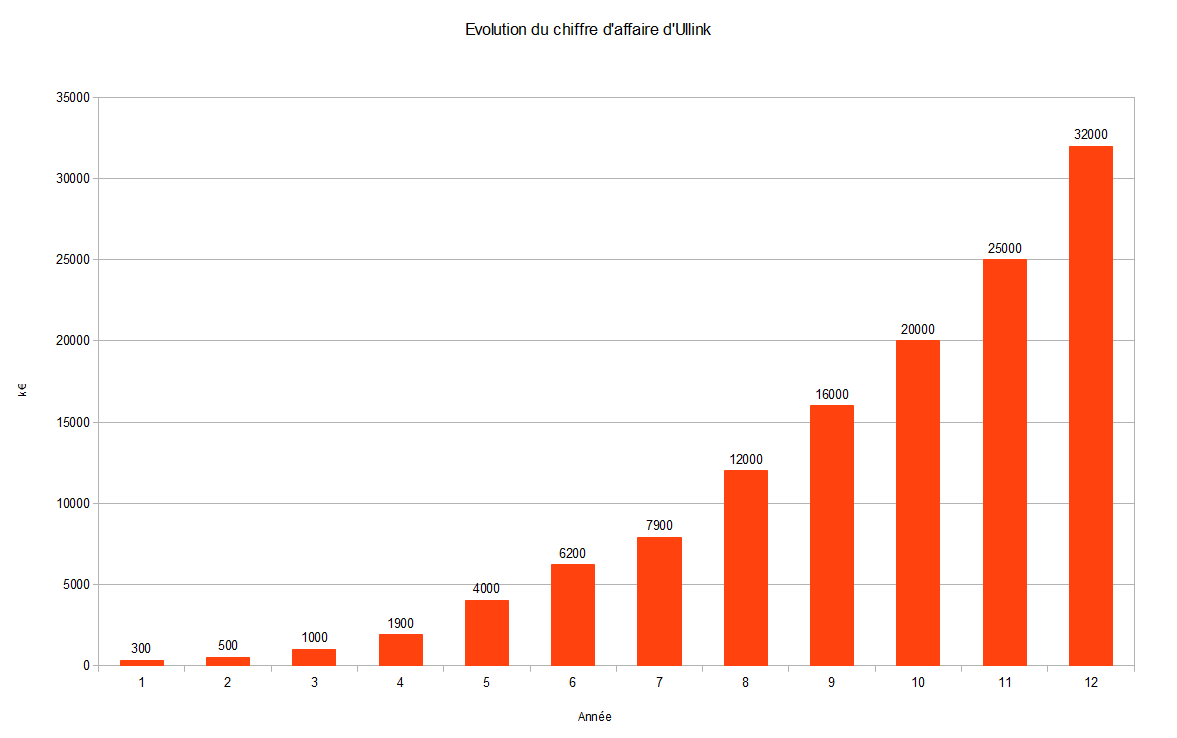
\includegraphics[width=\textwidth]{ca_ullink.png}

\subsection{Produits}

Ullink propose un ensemble de logiciels de trading électronique ayant pour cible l'ensemble des acteurs, aussi bien coté vente que achat. L'accent est mis sur la robustesse et l'extensibilité.

Trois types de produits sont ainsi proposés, que nous allons voir dans les paragraphes suivants.

\subsubsection{UL Desk}

UL Desk est la solution front-end pour tous les professionnels du marché, surtout les actions complexes, comme répartir un ordre entre plusieurs marchés, etc. C'est une interface tout inclus permettant un niveau d'abstraction par rapport aux marchés.

\subsubsection{Solutions complémentaires}
Un certain nombre d'autres composants logiciels sont disponibles pour offrir un ensemble de fonctionalités plus riche:

\begin{itemize}
\item{{\bf UL Bridge} permet la connexion client/marché(s) ainsi que le routage des informations dans l'ensemble des produits des solutions Ullink.}
\item{{\bf UL Odisys}: effectue une gestoin des ordres passés aux marchés, comme l'éclatement d'un ordre sur plusieurs marchés.}
\item{{\bf UL Smart} est une couche d'automatisation permettant l'automatisation des meilleures pratiques lors des passages d'ordres.}
\item{{\bf UL Iris} implémente une gestion des risques avant le passage réel d'un ordre sur les marchés.}
\item{{\bf UL Dashboard} permet d'avoir une vision d'ensemble de l'intégralité des activités réalisée sur la plateforme Ullink.}
\end{itemize}

\subsubsection{Hébergement}

Ullink propose ses produits sous la forme d'un service managé, c'est à dire géré par Ullink, et mis à disposition du client via une connexion à distance. Ce type de solution présente l'avantage pour le client de ne pas avoir à se soucier des inconvénients liés à la gestion d'une solution logicielle, tels que les mises à jour, le choix des machines, etc\dots

\subsection{Organisation}

Ullink est divisé en quatre départements majeurs:

\begin{itemize}
\item Produits\\
Tout ce qui concerne les produits Ullink, de l'architecture à la démarche qualité, en passant par le développement.

\item Opérations\\
Ce département est celui qui s'occupe des clients: réalistation de solutions, installation, support, gestion de portefeuille.

\item Business Development\\
Secteur marketing, vision stratégique...

\item Services internes\\
Comptabilité, RH, direction, IT interne.
\end{itemize}

\section{Activité au sein d'Ullink}

\subsection{Situation}

Je suis dans le département produit. Je forme avec mon camarade Sébastien ANTOINE, en IR3, l'équipe des Product tools. Nous sommes basés à Paris, dans un Open Space situé dans un immeuble du \textsc{\romannumeral 9}\textsuperscript{e}~arrondissement (voir Annexe 2).

Cette équipe se charge du développement et du maintien de l'environnement de travail propre au département Produit.

Lors des jeunes années d'Ullink, un environnement de travail basé sur de l'intégration continue a été mis en place. Cet environnement faisait usage de plusieurs outils open source, dont le désormais célèbre serveur Hudson, forké par la suite sous le nom Jenkins. Ce serveur interragissait avec un serveur CVS, via un plugin modifié installé sur Jenkins. Ce plugin se chargeait aussi de gérer les scripts ant, permettant la construction des solutions.

Cependant, ce qui était simple s'est complexifié avec le temps, le nombre de produits grandissant, les solutions spécifiques à tel client. L'équipe des Product Tools a donc été créée dans ce but: assurer la maintenance, et l'amélioration de ce système.

Dans ce cadre, nos sommes en contact avec toutes les différentes équipes produit.

\subsection{Missions}

\pagebreak
\begin{abstract}
Ceci est l'abstract
\end{abstract}

\end{document}
